\documentclass{article}
\usepackage[utf8]{inputenc}
\usepackage{geometry}
\usepackage{pgfplots}
\usepackage{graphicx}
\usepackage{verbatim}
\usepackage{amssymb}
\usepackage{amsmath}
\usepackage{tcolorbox} %needed
\usepackage{physics}
\usepackage{multicol}
\tcbuselibrary{listingsutf8}
\newcommand{\cls}{^{\circ}}


\geometry{a4paper, left=2cm, right=2cm, top=1cm, bottom=2cm}
\pgfplotsset{compat=1.18}

\begin{document}
I ¿Por qué, después de un rato de haber entrado a una alberca con agua fría, dejas de “sentir frío”?\\
\textit{Al entrar en contacto con el agua fría los dos sistemas (cuerpo y agua) que eran antes ajenos (o más bien con afectación termodinámica imperceptible) experimentan una transferencia de calor desde el cuerpo hacia el agua. En principio la diferencia de temperatura entre el cuerpo y el agua puede ser muy grande lo que provoca una sensación de frío, esto motivado también por la conductividad térmica de los sistemas. Sin embargo, a medida que el tiempo pasa adentro de la alberca la transferencia de calor sigue siendo continúa, pero a una tasa decreciente, pues la diferencia de temperatura $\Delta T$ entre el cuerpo y el agua se reduce gradualmente.}
\\\\


II. ¿Qué diferencia hay entre calor latente y calor específico?
\textit{El calor específico de una sustancia es la cantidad de calor que se necesita para elevar la temperatura de una unidad de masa de esa sustancia en una unidad de temperatura. Se expresa comúnmente en $ \frac{J}{kg \cdot \cls K} $ o $ \frac{cal}{g \cdot \cls C} $, pero siempre mantiene unidades de la forma $ \frac{Energia}{Masa \cdot Temperatura }$. Puede decirse que el calor específico indica la capacidad de una sustancia para almacenar calor que a diferencia del calor latente este actua sin experimentar un cambio de fase sino por un cambio de temperatura.} \\

\textit{El calor latente en cambio es la cantidad de energía térmica que se necesita para cambiar la fase de una unidad de masa de una sustancia sin cambiar su temperatura, en una gráfica T vs t podemos observar que e algún punto se vuelve isotérmico, es ahí donde este calor latente juega su rol pues aparece al no haber cambios de temperatura y estar ocurriendo un cambio de fase. Este calor que se libera o absorbe durante un cambio de fase a temperatura constante, se mide comúnmente en julios por kilogramo $\frac{J}{kg}$ en el SI o KMS, pero en general las unidades se rigen de la forma $\frac{Energia}{Masa}$. El calor latente es una medida de la energía necesaria para romper o formar enlaces moleculares sin cambiar la temperatura; ambos de ellos son usados para el cálculo del calor de un sistema, así que las unidades tan "fraccionarias" se deben a que cancela las unidades de masa que acompañan al calor latente/específico y en el caso del calor específico también cancelar la unidad de temperatura} \\\\

III. Calcular la magnitud de la fuerza que se obtiene en el émbolo mayor de una prensa hidráulica de un diámetro de 40 cm, si el émbolo menor de 20cm de diámetro se ejerce una fuerza de 700N. \\
\textit{Primero analizamos el sistema referente al émbolo menor, para ello ocupamos la ecuación de la presión.}
\begin{equation}
    P = \frac{F_m}{A_m} = \frac{4F_m}{\pi d_m^2}
\end{equation}
\textit{Hacemos algo análogo para el émbolo mayor donde con las sustituciones indicadas podemos obtener la fuerza, nótese que la presión en ese sistema al menos en nuestro punto de interés es la misma que la calculada por el émbolo menor.}
\begin{equation*}
    F_M = P \cdot A_M = \frac{4F_m}{\pi d_m^2} \cdot \frac{\pi d_M^2}{4}
\end{equation*}
\textit{Esto ya es totalmente automático de resolver, colocamos los valores que nos proporciona el enunciado considerando $20cm=0.2m$ y por ende $40cm=0.4m$}
\begin{equation*}
    F_M = \frac{4 \cdot 700N}{\pi (0.20cm)^2} \cdot \frac{\pi (0.40cm)^2}{4} = \frac{700 \cdot 0.40^2}{0.20^2} N =  2,800N
\end{equation*}
\\\\
IV. Si el acero es mucho más pesado que el agua, ¿por qué flotan los barcos?\\
\textit{La fuerza de flotación de un objeto en un líquido está determinada por la relación entre la densidad del objeto y la densidad del líquido. Según el principio de Arquímedes, un objeto flota en un líquido si su densidad es menor que la densidad del líquido en el que está sumergido, esto nos debería (en teoría) decir que el barco se hunde, pero esto es porque no se ha analizado completamente. Cuando se sumerge un objeto en un líquido, este desplaza una cierta cantidad de líquido lo que crea una fuerza de flotación $F_f$ hacia arriba igual al peso del líquido que ha sido desplazado, si el peso del objeto es menor que el peso del líquido desplazado entonces el objeto flotará. Aunque el acero es más pesado que el agua debido a la forma de los barcos y a la distribución de la masa es que pueden aprovecharse de este "principio de flotabilidad" pues los barcos están diseñados para tener una forma que les permita desplazar una gran cantidad de agua, al menos la suficiente para crear una fuerza de flotación suficiente para contrarrestar su peso. Para terminar, los barcos están huecos en su interior lo cual reduce su densidad efectiva y contribuye a su capacidad de flotación.}

\newpage
V. Un gas a 35°C y una presión de 440mm de Hg, se calienta hasta que su presión llega a 760 mm de Hg. Si el volumen permanece constante, ¿Cuál es la temperatura final del gas en °C? \\
\textit{Por el enunciado sabemos que es un sistema isocórico por lo que podemos emplear la ecuación de la Ley de Gay-Lussac o bien la ley combinada de los gases, aunque el volumen se eliminará de ambos lados por ser el mismo, utilizaremos la primera.}
\begin{equation}
    \frac{P_i}{T_i} = \frac{P_f}{T_f} \quad \Rightarrow \quad T_f = \frac{P_f}{P_i} \cdot T_i
\end{equation}
\textit{Ahora solo sustituimos, nótese que no nos afectan las unidades en los cálculos pues la razón de las presiones es adimensional y la temperatura incial está expresada en Celsius tal cual requiere el enunciado.}
\begin{equation*}
    T_f = \frac{P_f}{P_i} \cdot T_i = \frac{760 mmHg}{440 mmHg} \cdot 35 \cls C = 60.45454 \cls C
\end{equation*}

VI. ¿Cuál es el cambio en la energía interna de un sistema si se le suministran 700cal de energía en forma de calor, y se le aplica un trabajo de 900 Joules?\\
\textit{Si le suministra calor y se le realiza trabajo al sistema estas energías \textbf{adquieren} signo positivo, he resaltado "adquieren" pues en el caso del trabajo consideraremos $W=-900$, pero esto es por nuestra convención de signos en la ecuación de la energía interna ya que W sería 900 si el sistema fuese quien está realizando este trabajo, no medios externos, finalmente adquirirá un valor positivo.}
\begin{equation*}
    \Delta U = Q - W = 700cal + 900J = 700cal \cdot \frac{4.184J}{1cal} + 900J = 3,828.8 J
\end{equation*}
\\\\
VII. El agua dentro de un recipiente se presuriza con aire y la presión se mide con un manómetro de varios fluidos como se muestra en Figure I. Determina la presión manométrica del aire en el recipiente
si $h_1 = 0.2m$, h2 = 0.3m y h3= 0.46m. Considere las densidades del agua (1,000 kg/m3), del aceite (850 kg/m3) y del mercurio (13,600 kg/$m^3$). \\
\textit{Utilizaremos las variables que están contenidas en el dibujo. Es complicado explicar este problema en líneas de texto pues se necesita continuamente hacer referencias al dibujo por lo que en varias ocasiones ocuparé lenguaje informal en un intento de describir el fenómeno; vemos que la presión atmosférica es igual al conjunto de presiones que constituye al sistema, desde el punto 2 hasta el punto 1 que es en donde se encuentra el aire y lo que queremos despejar. \\}
\textit{Empezaremos a analizar el sistema desde el punto 1, aumenta la presión del agua en la altura $h_1+h_2$ por "bajar" pero se contrarresta parcialmente al tener que subir por el tubo delgado una altura $h_2$, por lo que la presión del agua se determina por $h_1+h_2-h_2=h_1$; el aceite sube una altura $h_1$ por lo que disminuye su presión, y después sube una altura desconocida, no nos importa pues en ese límite de $h_1$ en el tubito de la izquierda del aceite y en el tubito de la derecha del aceite la presión es la misma, de hecho el razonamiento correcto es considerar esta propiedad física desde $h_2$ pues sube y baja la presión en función de $h_1+?-?-h_1=0$, el aceite solo termine bajando $h_2$ así que en este tramo la presión del aceite se determina por $h_2$; finalmente el tramo del mercurio es evidente que solo se determina por $h_3$ pues la presión en su punto de partida y en el tubito de la izquierda con la misma altura es igual, así que solo se considera que subió $h_3$ que es la única presión negativa de todo lo que hemos calculado. Es así que usando la ecuación de presión manométrica obtenemos lo siguiente.}
\begin{align*}
    P_{man} &= P_1 - P_{atm} \\
    &= P_1 - [P_1 + \rho_{h20} g h_1 + \rho_{ac} g h_2 - \rho_{hg} g h_3] \\
    &= \rho_{hg} g h_3 - \rho_{h20} g h_1 - \rho_{ac} g h_2 \\
    &= 9.806\frac{m}{s^2}(13,600kg/m^3 \cdot 0.46m - 1,000kg/m^3 \cdot 0.2m - 850kg/m^3 \cdot 0.3m) \\
    &\approx 56,884.606 \frac{kgm}{s^2} \cdot \frac{1}{m^2} = 56,884.606 Pa
\end{align*}

\begin{figure}[h]
    \centering
    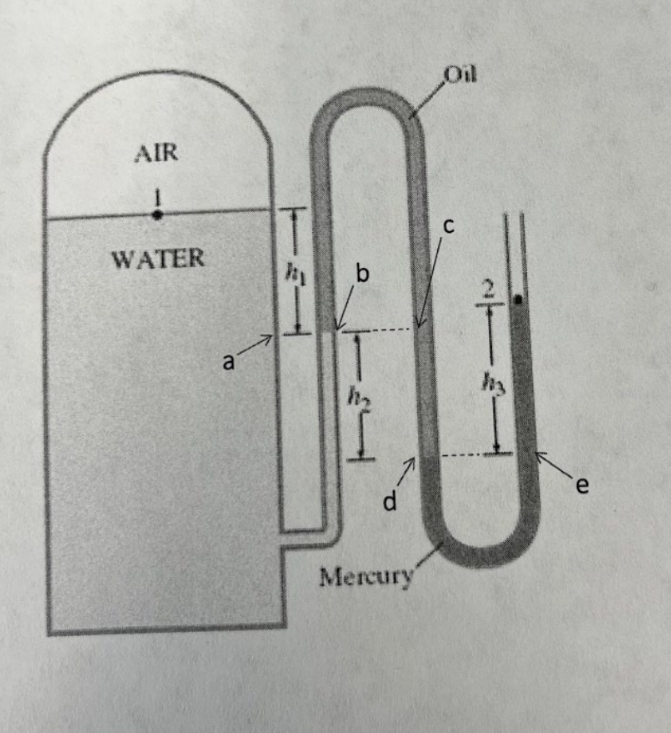
\includegraphics[width=0.15\linewidth]{VII.png}
    \caption{Visualización del ejercicio VII}
    \label{fig:enter-label}
\end{figure}

\end{document}